% Template file for an a0 landscape poster.
% Written by Graeme, 2001-03 based on Norman's original microlensing
% poster.
%
% See discussion and documentation at
% <http://www.astro.gla.ac.uk/users/norman/docs/posters/>
%
% $Id: poster-template-landscape.tex,v 1.2 2002/12/03 11:25:46 norman Exp $


% Default mode is landscape, which is what we want, however dvips and
% a0poster do not quite do the right thing, so we end up with text in
% landscape style (wide and short) down a portrait page (narrow and
% long). Printing this onto the a0 printer chops the right hand edge.
% However, 'psnup' can save the day, reorienting the text so that the
% poster prints lengthways down an a0 portrait bounding box.
%
% 'psnup -w85cm -h119cm -f poster_from_dvips.ps poster_in_landscape.ps'

\documentclass[a0]{a0poster}
% You might find the 'draft' option to a0 poster useful if you have
% lots of graphics, because they can take some time to process and
% display. (\documentclass[a0,draft]{a0poster})

\pagestyle{empty}
\setcounter{secnumdepth}{0}

% The textpos package is necessary to position textblocks at arbitary
% places on the page.
\usepackage[absolute]{textpos}

% Graphics to include graphics. Times is nice on posters, but you
% might want to switch it off and go for CMR fonts.
\usepackage{graphics,graphicx,wrapfig,times,amssymb,amsfonts,amsthm}

% These colors are tried and tested for titles and headers. Don't
% over use color!
\usepackage{color}
\definecolor{DarkBlue}{rgb}{0.1,0.1,0.5}
\definecolor{Red}{rgb}{0.9,0.0,0.1}
\definecolor{DarkBlue}{rgb}{0.1,0.1,0.5}
\definecolor{DarkGreen}{rgb}{0.0,0.4,0.0}
%%%%%%%%%%%%%%%%%%%%%%%%%%%%%%%%%%%%%
\newtheorem{theorem}{Theorem}
\newtheorem{corollary}{Corollary}
\newtheorem{lemma}{Lemma}
\newtheorem{proposition}{Proposition}
\theoremstyle{definition}
\newtheorem{example}{Example}
\newtheorem{definition}{Definition}
%%%%%%%%%%%%%%%%%%%%%%%%%%%%%%%%%%%%%%%%%%%%%%%%%%%%%%%%%%%%%%%%%%%%%%%%%%%%%%%%%%%%%%%%%%%%
% see documentation for a0poster class for the size options here
\let\Textsize\normalsize
\def\RHead#1{\noindent\hbox to \hsize{\hfil{\bf \LARGE\color{DarkBlue} #1}}\smallskip}
\def\LHead#1{\noindent{\bf \LARGE\color{DarkBlue} #1}\smallskip}
\def\LHeadGreen#1{\noindent{\bf \LARGE\color{DarkGreen} #1}\smallskip}
\def\CHead#1{\noindent\hbox to \hsize{\hfil{\bf \LARGE\color{DarkBlue} #1}\hfil}\smallskip}
\def\Subhead#1{\noindent{\large\color{DarkBlue} #1}}
\def\Title#1{\noindent{\VERYHuge\color{Red} #1}}
\newcommand\doubleline{\hrule\ \vspace{-10pt} \hrule}
% Next line controls interline spacing. 1 = single space
\renewcommand{\baselinestretch}{1.5}
%%%%%%%%%%%%%%%%%%%%%%%%%%%%%%%%%%%%%%%%%%%%%%%%%%%%%%%%%%%%%%%%%%%%%%%%%%%%%%%%%%%%%%%%%%%%
% SOME USER DEFINED ITEMS
\newcommand{\dis}{\displaystyle}
\newcommand{\reals}{\mathbb{R}}
\newcommand{\naturals}{\mathbb{N}}
\newcommand{\integers}{\mathbb{Z}}
\newcommand{\rationals}{\mathbb{Q}}
\newcommand{\complex}{\mathbb{C}}
% Set up the grid
%
% Note that [40mm,40mm] is the margin round the edge of the page --
% it is _not_ the grid size. That is always defined as
% PAGE_WIDTH/HGRID and PAGE_HEIGHT/VGRID. In this case we use
% 23 x 12. This gives us three columns of width 7 boxes, with a gap of
% width 1 in between them. 12 vertical boxes is a good number to work
% with.
%
% Note however that texblocks can be positioned fractionally as well,
% so really any convenient grid size can be used.
%
\TPGrid[40mm,40mm]{23}{12}      % 3 cols of width 7, plus 2 gaps width 1

\parindent=0pt
\parskip=0.5\baselineskip

\begin{document}

% Understanding textblocks is the key to being able to do a poster in
% LaTeX. In
%
%    \begin{textblock}{wid}(x,y)
%    ...
%    \end{textblock}
%
% the first argument gives the block width in units of the grid
% cells specified above in \TPGrid; the second gives the (x,y)
% position on the grid, with the y axis pointing down.

% You will have to do a lot of previewing to get everything in the
% right place.

% This gives good title positioning for a portrait poster.
% Watch out for hyphenation in titles - LaTeX will do it
% but it looks awful.
%%%%%%%%%%%%%%%%%%%%%%%%%%%%%%%%%%%%%%%%%%%%%%%%%%%%%%%%%%%%%%%%%
%%%%%%%%%%%%%%%%%%%%%%%%%%%%%%%%%%%%%%%%%%%%%%%%%%%%%%%%%%%%%%%%%
% HERE BEGINS THE DOCUMENT PROPER

%%%%%%%%%%%%%%%%%%%%%%%%%%%%%%%%%%%%%%%%%%%%%%%%%%%%%
% Title                                             %
% The title at coordinates (0,-0.35)                %
%%%%%%%%%%%%%%%%%%%%%%%%%%%%%%%%%%%%%%%%%%%%%%%%%%%%%
\begin{textblock}{23}(0,-0.35)
\begin{center}
\Title{The Wonderful Arithmetic Aspects of Elementary Functions}
\end{center}
\end{textblock}

%%%%%%%%%%%%%%%%%%%%%%%%%%%%%%%%%%%%%%%%%%%%%%%%%%%%%
% Authors                                           %
%%%%%%%%%%%%%%%%%%%%%%%%%%%%%%%%%%%%%%%%%%%%%%%%%%%%%
\newcommand{\firstauthor}{Carl F. Gauss}
\newcommand{\firstauthoruni}{G\"ottingen University}
\newcommand{\firstauthoremail}{gauss@msri.org}
%%%%%%%%%%%%%%%%%%%%%%%%%%%%%%%%%%%%%%%%%%%%%%%%%%%%%
\newcommand{\secondauthor}{Leonhard Euler}
\newcommand{\secondauthoruni}{Basel College}
\newcommand{\secondauthoremail}{euler@basel.edu}
%%%%%%%%%%%%%%%%%%%%%%%%%%%%%%%%%%%%%%%%%%%%%%%%%%%%%
\newcommand{\thirdauthor}{Emmy N\"oether}
\newcommand{\thirdauthoruni}{Berlin Academy}
\newcommand{\thirdauthoremail}{noether@berlin.de}
%%%%%%%%%%%%%%%%%%%%%%%%%%%%%%%%%%%%%%%%%%%%%%%%%%%%%
\begin{textblock}{7}(0,0.25)
\begin{center}
{\color{DarkBlue}\LARGE
% This is where the first author is printed
\firstauthor}\\
{\color{DarkBlue}\Large{\it \firstauthoruni}}
\end{center}
\end{textblock}
%%%%%%%%%%%%%%%%%%%%%%%%%%%%%%%%%%%%%%%%%%%%%%%%%%%%%%%%%
\begin{textblock}{7}(8,0.25)
\begin{center}
{\color{DarkBlue}\LARGE
% This is where the second author is printed
\secondauthor}\\
{\color{DarkBlue}\Large{\it \secondauthoruni}}
\end{center}
\end{textblock}
%%%%%%%%%%%%%%%%%%%%%%%%%%%%%%%%%%%%%%%%%%%%%%%%%%%%%%%%%
\begin{textblock}{7}(16,0.25)
\begin{center}
{\color{DarkBlue}\LARGE
% This is where the third author is printed
\thirdauthor}\\
{\color{DarkBlue}\Large{\it \thirdauthoruni}}
\end{center}
\end{textblock}
%%%%%%%%%%%%%%%%%%%%%%%%%%%%%%%%%%%%%%%%%%%%%%%%%%%%%%%%%
% The next few lines are for the double line under the  %
% title and authors.                                    %
%%%%%%%%%%%%%%%%%%%%%%%%%%%%%%%%%%%%%%%%%%%%%%%%%%%%%%%%%
\begin{textblock}{23}(0,0.78)
\begin{center}
\smallskip
\doubleline
\end{center}
\end{textblock}
%%%%%%%%%%%%%%%%%%%%%%%%%%%%%%%%%%%%%%%%%%%%%%%%%%%%%
% MSRI-UP Logo                                      %
% It is at the upper right corner                   %
%%%%%%%%%%%%%%%%%%%%%%%%%%%%%%%%%%%%%%%%%%%%%%%%%%%%%
\begin{textblock}{2}(22,-0.25)
\resizebox{1.5\TPHorizModule}{!}{
\includegraphics{MSRI_Logo.png}}
\end{textblock}
%%%%%%%%%%%%%%%%%%%%%%%%%%%%%%%%%%%%%%%%%%%%%%%%%%%%%
% COLUMN 1                                          %
% The top of column 1 is at coordinates (0,1.0)     %
%%%%%%%%%%%%%%%%%%%%%%%%%%%%%%%%%%%%%%%%%%%%%%%%%%%%%
\begin{textblock}{7}(0,1.0)
%%%%%%%%%%%%%%%%%%%%%%%%%%%%%%%%%%%%%%%%%%%%%%%%%%%%%
% Abstract                                          %
%%%%%%%%%%%%%%%%%%%%%%%%%%%%%%%%%%%%%%%%%%%%%%%%%%%%%
\LHead{Abstract}\\
% Enter abstract here
We present a sequence of polynomials in $\mathbb{Q}[x]$, arising
from a simple family of rational functions, that approximates
uniformly the classical function $\arctan x$ on $[0,1]$ (and hence,
via standard identities, on all of $\mathbb{R}$).  The sequence is
attractive and interesting for several reasons including its rate of
convergence, its simplicity, its rational approximations to $\pi$, and
because of its similarities with Hermite-interpolating polynomials.
\medskip
\hrule
\end{textblock}
%%%%%%%%%%%%%%%%%%%%%%%%%%%%%%%%%%%%%%
\begin{textblock}{7}(0,2.75)
\LHead{Introduction}\\
The Taylor series
$$ \arctan x = x - \frac{x^3}{3} + \frac{x^5}{5} - +
\cdots = \sum_{k=0}^\infty \frac{(-1)^k}{2k+1}\, x^{2k+1}$$
was discovered by the Scotsman James Gregory in 1671 (\cite[Ch.\thinspace12]{B}).
It is not hard to show that the
series converges uniformly to $\arctan x$ on
$[-1,1]$; thus, the series produces the
following sequence of Taylor polynomials in $\mathbb{Q}[x]$
that converges uniformly to $\arctan x$
on $[-1,1]$:
$$T_n(x) = \sum_{k=0}^n \frac{(-1)^k}{2k+1}\, x^{2k+1}.$$

Like the Taylor polynomials for several other classical functions, e.g.,
$\cos x,\ \sin x,$ and $e^x$, this sequence of polynomials is very easy to describe and
work with; but unlike those Taylor polynomials with factorials in the denominators of their
coefficients, it does not converge rapidly for all ``important" values of $x$.
In particular, it converges extremely slowly to $\arctan x$ when $|x|$ is near $1$.
For example, if $x=0.95$, we would need to use
$T_{28}$, a polynomial of degree $57$, to get three decimal places of
accuracy for $\arctan (0.95)$; if $x=1$, we would need to use
$T_{500}$, a polynomial of degree $1001$, to get three decimal places
of accuracy for $\arctan 1$.

Indeed, for $x\in[0,1]$
\begin{eqnarray*}
\arctan x &=& \int_0^x \frac{1}{1+t^2}\,dt \\
&=& \int_0^x \sum_{k=0}^\infty (-1)^k\, t^{2k}\,dt\\
&=&\int_0^x \sum_{k=0}^n (-1)^k\, t^{2k} + \sum_{k=n+1}^\infty (-1)^k\, t^{2k}\,dt\\
&=&T_n(x) + (-1)^{n+1} \int_0^x \frac{t^{2n+2}}{1+t^2}\,dt;
\end{eqnarray*}
therefore, $\dis|\arctan x - T_n(x)| = \int_0^x \frac{t^{2n+2}}{1+t^2}\,dt
\geq \int_0^x \frac{t^{2n+2}}{2}\,dt = \frac{x^{2n+3}}{2(2n+3)}$.
Thus, as $x\to 1$, $T_n(x)$ cannot approximate $\arctan x$ any better
than $\frac{1}{2(2n+3)} = \frac{1}{2({\rm degree\ }T_n) + 4}$.
The same holds true for $x$ values near $-1$. It is only fair to note that the sequence
$\{T_n(x)\}$ converges to $\arctan x$ reasonably
fast for $x$ values near $0$.

The purpose of this article is to present  another very elementary,
easily-described
sequence of polynomials in $\mathbb{Q}[x]$
that approximates $\arctan x$ uniformly on $[0,1]$
and which does so much more rapidly than the sequence of
Taylor polynomials centered at $0$. We note that
such an approximating sequence provides,
via the identities $\arctan x = -\arctan (-x)=\frac{\pi}{2} -
\arctan (\frac{1}{x})$, a method of approximating $\arctan x$ for
all $x\in\mathbb{R}$.
The approximating sequence arises from the simple family of rational functions
$\dis\Big\{\frac{x^{4m}(1-x)^{4m}}{1+x^2}\Big\}_{m\in\mathbb{N}}$.
\end{textblock}

%%%%%%%%%%%%%%%%%%%%%%%%%%%%%%%%%%%%%%%%%%%%%%%%%%%%%
% COLUMN 2                                          %
% The top of column 2 is at coordinates (8,1.0)     %
%%%%%%%%%%%%%%%%%%%%%%%%%%%%%%%%%%%%%%%%%%%%%%%%%%%%%
\begin{textblock}{7}(8,1.0)
\LHead{Results}\\
Indeed, because of Theorem \ref{basicrecursion}, the sequence $\{h_m\}$ is easily programmable
and gives functions that will approximate $\arctan$ to a prescribed
accuracy for $x\in [0,1]$. Appendix A contains a {\sl Mathematica} program
that computes the necessary $h_m(x)$ to approximate $\arctan x,\ x\in[0,1],$ to
``{\tt numberofdigits}" decimal places of accuracy.
The program computes the $h_m$ much faster than the direct
computation of the coefficients, via solving a system of linear equations,
suggested by the result of Theorem \ref{basicrecursion}. For example,
to find a polynomial $h_m$ of degree $8m$ such that $h_m(0)=\arctan 0$,
$h_m^{(n)}(0) = \arctan^{(n)}(0)$ and $h_m^{(n)}(1) = \arctan^{(n)}(1)$ for
$1\leq n \leq 4m$, we solved for the coefficients of $h_m$ by solving
the system of linear equations (the $8m+1$ coefficients being
the unknown variables),
generated by the conditions on $h_m$. For
$m=5,\ 10,\ 15,$ and $20$, on a 733 MHz Pentium III computer running
{\sl Mathematica} $4.1$,  this method yielded computation times of $0.82,\ 13.63,\ 88.1\ $ and $332.08$ seconds respectively. The program above
(without the ``Print" statements)
computed the $h_m$ in $0.0,\ 0.06,\ 0.11$ and $0.11$ seconds respectively.

\begin{lemma}\label{basicrecursion}
Define $p_1(x) = 4-4x^2+5x^4-4x^5+x^6$ and $p_m(x)
= x^4 (1-x)^4 p_{m-1}(x) + (-4)^{m-1} p_1(x)$ for $m\geq 2$. Then
$$\frac{x^{4m} (1-x)^{4m}}{1+x^2} = p_m(x) + \frac{(-4)^m}{1+x^2},
\ {\rm for\ all\ }m\in\mathbb{N}.$$
\end{lemma}

\begin{proof}
We argue by induction on $m$. A computation shows that $\frac{x^4 (1-x)^4}{1+x^2} =
p_1(x) - \frac{4}{1+x^2}$. Assume $\frac{x^{4m} (1-x)^{4m}}{1+x^2} = p_m(x) +
\frac{(-4)^m}{1+x^2}$. Now
\begin{eqnarray*}
\frac{x^{4(m+1)}\ (1-x)^{4(m+1)}}{1+x^2} &=&
x^4 (1-x)^4 \Big( p_m(x) + \frac{(-4)^m}{1+x^2} \Big)\\
&=& x^4 (1-x)^4  p_m(x) + (-4)^m \frac{x^4 (1-x)^4}{1+x^2}\\
&=& x^4 (1-x)^4  p_m(x) + (-4)^m \Big(p_1(x) - \frac{4}{1+x^2}\Big)\\
&=& x^4 (1-x)^4  p_m(x) + (-4)^m p_1(x) + \frac{(-4)^{m+1}}{1+x^2}\\
&=& p_{m+1}(x) + \frac{(-4)^{m+1}}{1+x^2}.\\
\end{eqnarray*}
\vskip-70pt
\end{proof}
\end{textblock}

%%%%%%%%%%%%%%%%%%%%%%%%%%%%%%%%%%%%%%%%%%%%%%%%%%%%%
% INSERTING A GRAPHIC                               %
% PDF files look and scale better so you            %
% probably want to convert your graphic from jpeg   %
% to pdf. You can do this using Adobe Acrobat.      %
%%%%%%%%%%%%%%%%%%%%%%%%%%%%%%%%%%%%%%%%%%%%%%%%%%%%%
\begin{textblock}{7}(8,8)
\begin{center}
\begin{figure}[h]
% options for \includegraphics are like
% 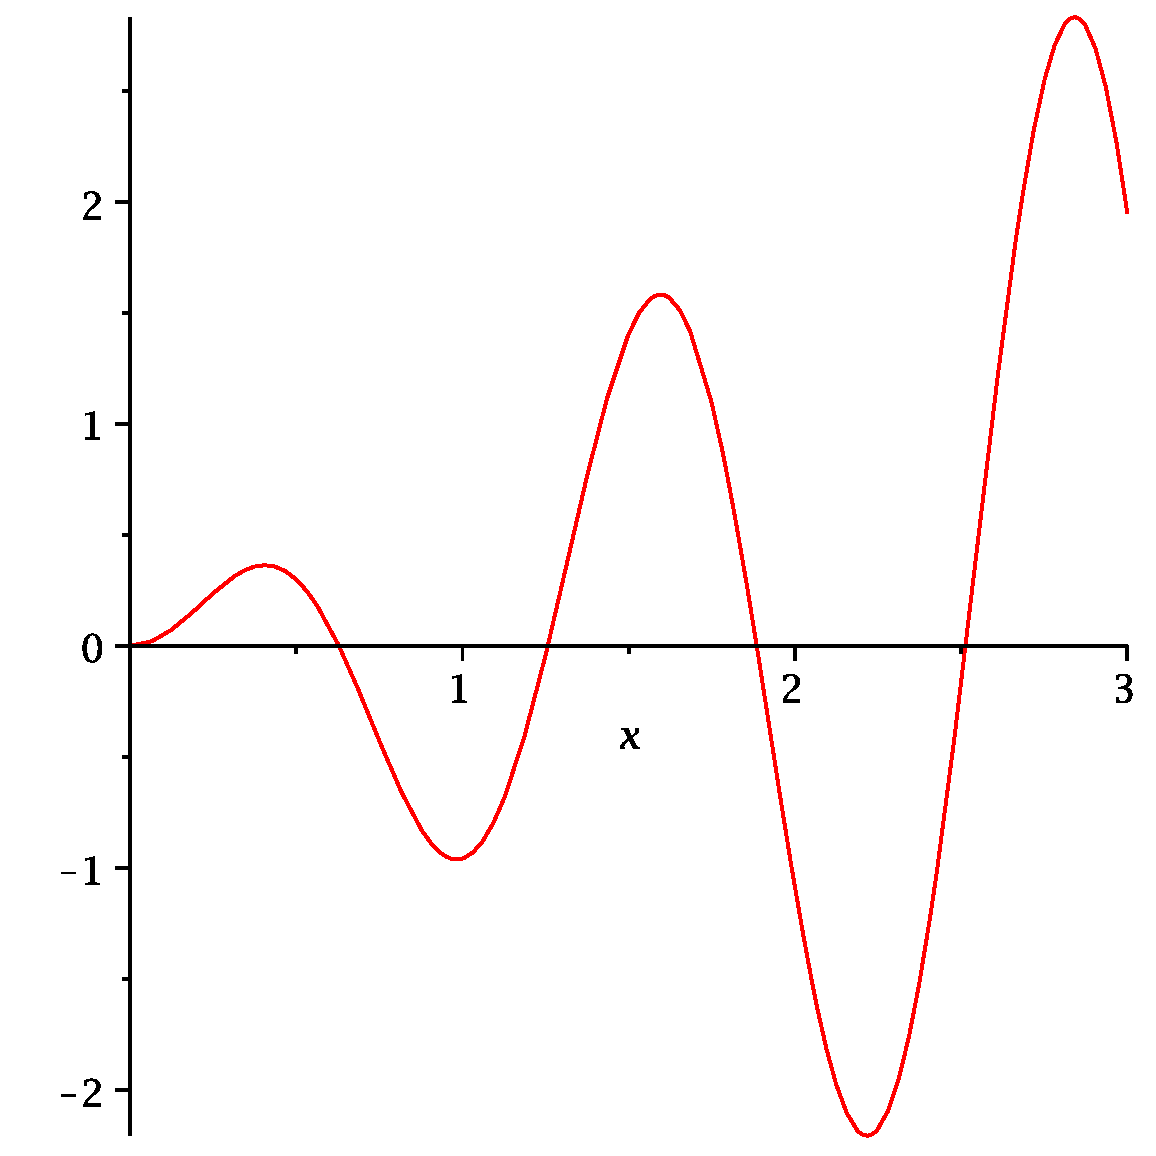
\includegraphics[angle=45,width=200mm,height=300mm]{sampleplot.pdf}
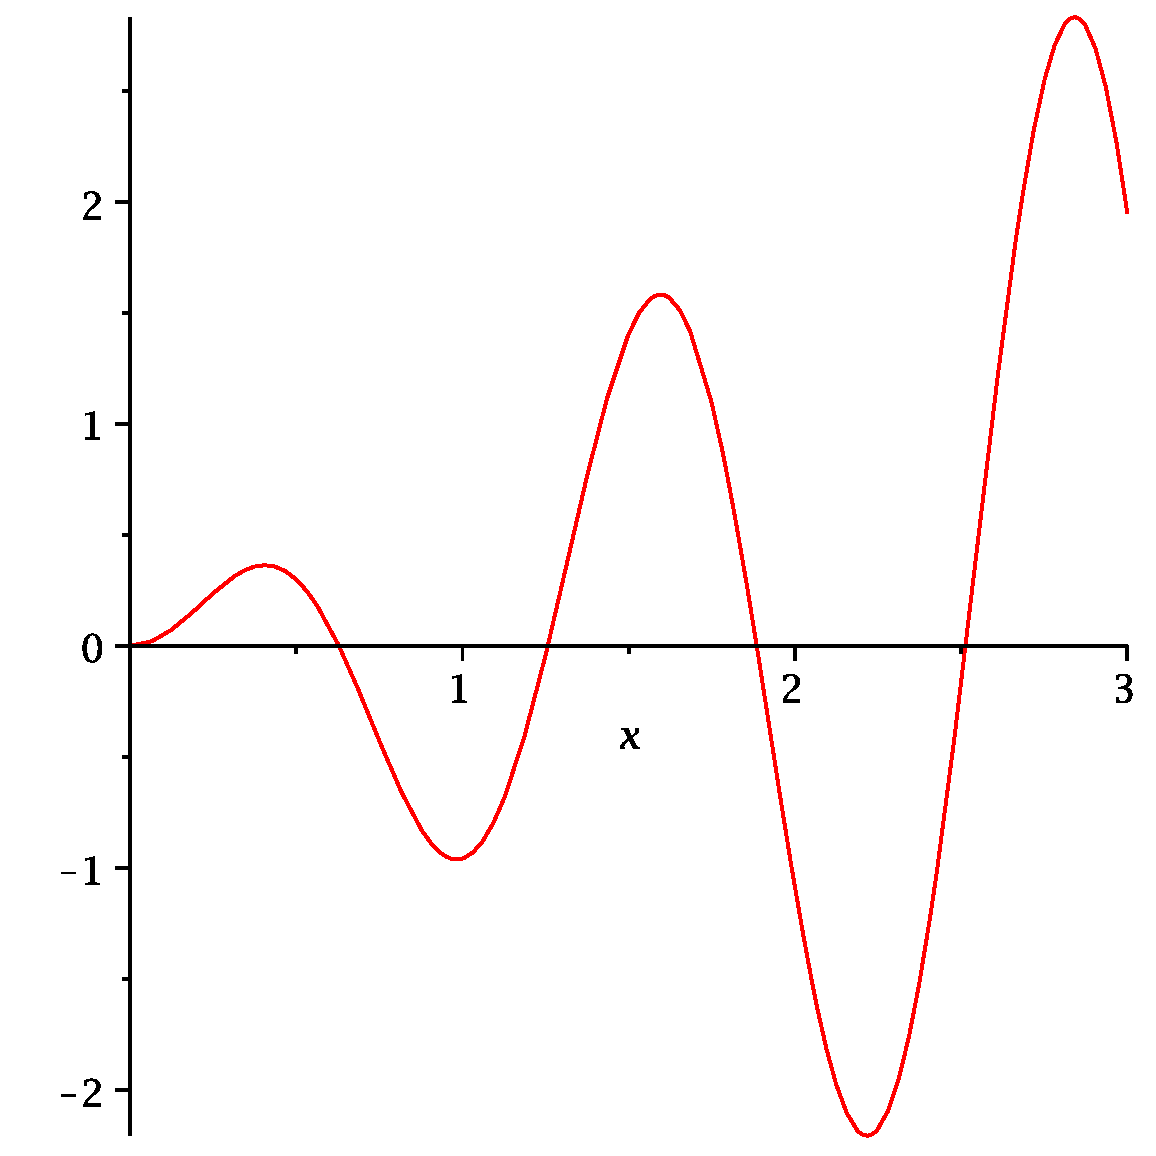
\includegraphics[width=200mm]{sampleplot.pdf}
\caption{An example graphic}
\label{graph:sample}
\end{figure}
\end{center}

\end{textblock}

%%%%%%%%%%%%%%%%%%%%%%%%%%%%%%%%%%%%%%%%%%%%%%%%%%%%%
% COLUMN 3                                          %
% The top of column 3 is at coordinates (16,1.0)    %
%%%%%%%%%%%%%%%%%%%%%%%%%%%%%%%%%%%%%%%%%%%%%%%%%%%%%
\begin{textblock}{7}(16,1.0)
\LHead{Conclusion}\\
Here are my primary conclusions.

\begin{theorem}\label{basictheorem}
Define $p_1(x) = 4-4x^2+5x^4-4x^5+x^6$ and $p_m(x)
= x^4 (1-x)^4 p_{m-1}(x) + (-4)^{m-1} p_1(x)$ for $m\geq 2$. Then
$$\frac{x^{4m} (1-x)^{4m}}{1+x^2} = p_m(x) + \frac{(-4)^m}{1+x^2},
\ {\rm for\ all\ }m\in\mathbb{N}.$$
\end{theorem}

\begin{proof}
We argue by induction on $m$. A computation shows that $\frac{x^4 (1-x)^4}{1+x^2} =
p_1(x) - \frac{4}{1+x^2}$. Assume $\frac{x^{4m} (1-x)^{4m}}{1+x^2} = p_m(x) +
\frac{(-4)^m}{1+x^2}$. Now
\begin{eqnarray*}
\frac{x^{4(m+1)}\ (1-x)^{4(m+1)}}{1+x^2} &=&
x^4 (1-x)^4 \Big( p_m(x) + \frac{(-4)^m}{1+x^2} \Big)\\
&=& x^4 (1-x)^4  p_m(x) + (-4)^m \frac{x^4 (1-x)^4}{1+x^2}\\
&=& x^4 (1-x)^4  p_m(x) + (-4)^m \Big(p_1(x) - \frac{4}{1+x^2}\Big)\\
&=& x^4 (1-x)^4  p_m(x) + (-4)^m p_1(x) + \frac{(-4)^{m+1}}{1+x^2}\\
&=& p_{m+1}(x) + \frac{(-4)^{m+1}}{1+x^2}.\\
\end{eqnarray*}
\vskip-70pt
\end{proof}

\end{textblock}
%%%%%%%%%%%%%%%%%%%%%%%%%%%%%%%%%%%%%%%%%%%%%%%%%%%%%%%%%%%%%%%%%%
% Bibliography                                                   %
% Coordinates (16,6) are good for the references                 %
% but this will depend on your content and number of references. %
%%%%%%%%%%%%%%%%%%%%%%%%%%%%%%%%%%%%%%%%%%%%%%%%%%%%%%%%%%%%%%%%%%
\begin{textblock}{7}(16,6)
\renewcommand\refname{{\LARGE\color{DarkBlue} References}}
\hrule
\begin{thebibliography}{aaaa}
\bibitem[B]{B}P. Beckmann, \textit{A History of Pi},
St. Martin's Press, New York, 1976.

\bibitem[BF]{BF}R.L. Burden \& J.D. Faires, \textit{Numerical Analysis}, 6th Ed., Brooks/Cole,
Pacific Grove, CA, 1997.

\bibitem[S1]{S}D. Smith, ``A Fortran Package For Floating-Point Multiple-Precision Arithmetic",
\textit{Transactions on Mathematical Software}, \textbf{17} (1991),
273 -- 283.

\bibitem[S2]{S2}D. Smith, ``Efficient Multiple-Precision Evaluation of
Elementary Functions", \textit{Mathematics of Computation},
\textbf{52} (1989), 131 -- 134.

%%%
%%%
\end{thebibliography}
\end{textblock}
%%%%%%%%%%%%%%%%%%%%%%%%%%%%%%%%%%%%%%%%%%%%%%%%%%%%%%%%%%%%%%%%%
% Acknowledgements                                              %
% Coordinates (16,9.5) are good for the acknowledgments         %
%%%%%%%%%%%%%%%%%%%%%%%%%%%%%%%%%%%%%%%%%%%%%%%%%%%%%%%%%%%%%%%%%
\begin{textblock}{7}(16,9.5)
\hrule
\LHeadGreen{Acknowledgements}\\
% Enter acknowledgements here
This research was conducted during the 2014 Mathematical Sciences Research Institute Undergraduate Program (MSRI-UP) in Berkeley, CA under the direction of Prof. Victor H. Moll, Tulane University. MSRI-UP is supported by the National Science Foundation (grant No. DMS-1156499) and the National Security Agency (grant No. H-98230-13-1-0262). We would like to thank ... 
\end{textblock}

%%%%%%%%%%%%%%%%%%%%%%%%%%%%%%%%%%%%%%%%%%%%%%%%%%%%%%%%%%%%%%%%%
% Contact Information                                           %
% Coordinates (16,11.5) are good for the contact information,   %
% but the 11.5 may need to be adjusted depending on length of   %
% references and acknowledgments. Info for authors entered      %
% automatically from above.                                     %
%%%%%%%%%%%%%%%%%%%%%%%%%%%%%%%%%%%%%%%%%%%%%%%%%%%%%%%%%%%%%%%%%
\begin{textblock}{7}(16,11.5)
\hrule
\Subhead{Contact Information}:\ \
\firstauthor: {\sl \firstauthoremail};
\secondauthor: {\sl \secondauthoremail};\\
\thirdauthor: {\sl \thirdauthoremail}
\end{textblock}


\end{document}
